\DiaryEntry{Single-Source Shortest Paths - Proofs (2)}{2020-05-12}{Algorithms}

\subsection{Proof of the Bellman-Ford Algorithm}

As a reminder, the Bellman-Ford algorithm looks like the following.

\begin{Verbatim}[numbers=left, xleftmargin=5mm]
Bellman-Ford(G, w, s)
   Init-Single-Source(G,s)
   for i = 1 to |G.V|-1
      for each edge (u,v) in G.E
         Relax(u,v,w)
   for each edge (u,v) in G.E
      if v.d > u.d + w(u,v)
         return false
   return true
\end{Verbatim}


\begin{theorem} Let $G = (V,E)$ be a weighted, directed graph with source $s$ and weight function $w: E \rightarrow \mR$, and assume that $G$ contains no neagtive-weight cycles reachable from $s$. Then after $|V|-1$ iterations of the for loop in line $3$ of \verb Bellman-Ford , we have $v.d = \delta(s,v)$ for all vertices $v$ that are reachable from $s$.
\end{theorem}

\begin{proof} We use the path-relaxation property: Consider a vertex $v$ reachable from $s$ and a shortest path (of length $k$) from $s$ to $v$: $p = \langle v_0 = s, v_1, \ldots, v_{k-1}, v_k = v \rangle$. Shortest paths are simple, therefore $p$ has at most $|V|-1$ edges and therefore $k \leq |V| -1$.  Each of the $|V|-1$ iterations of the for loop relaxes all $|E|$ edges. In the $i$-th iteration, the edge $(v_{i-1},v_i)$ is relaxed (among other edges). By the path relaxation property, we have $v.d = v_k.d = \delta(s, v_k) = \delta(s,v)$.
\end{proof}


\begin{theorem}[Correctness of Bellman-Ford Algorithm] We let the Bellman-Ford Algorithm run on a weighted, directed graph $G$. If $G$ contains no negative-weight cycles reachable from source vertex $s$, then the algorithm returns \verb true , we have $v.d = \delta(s, v)$ for all vertices $v \in V$, and the predecessor subgraph $G_\pi$ is a shortest-paths tree rooted at $s$. If $G$ contains negative-weight cyclesreachable from $s$, the algorithm returns \verb false .
\end{theorem}

\begin{proof}
  Suppose the graph $G$ does not contain negative-weight cycles reachable from source vertex $s$. If $v$ is reachable from $s$, then at termination we have $v.d = \delta(s,v)$ from the previous theorem. If $v$ is not reachable from $s$, then by the No-Path Property, we have $v.d = \infty$. In both cases, the predecessor-subgraph property implies that $G-\pi$ is a shortest-path tree rooted at $s$.

  Now we show that the algorithm returns \verb true : At termination, we have for all edges $(u,v) \in E$,

  \bee
  v.d = \delta(s,v) \leq \delta(s,u) + w(u,v) = u.d + w(u,v)
  \eee

  where the inequality follows from the triangle inequality. Therefore none of the tests in line $7$ returns \verb false .

  Now we consider the case that the graph contains a negative-weight cycles reachable from source vertex $s$. Let this cycle denote $c = \langle v_0, v_1, \ldots, v_k \rangle$ with $v_0 = v_k$. The definition of a negative-weight cycle implies that

  \begin{equation}\label{sssp3:eq-1}
  \sum_{i=1}^k w(v_{i-1}, v_i) < 0
  \end{equation}

  We use proof by contradiction and assume that the algorithm returns \verb true . Thus, $v_i.d \leq v_{i-1}.d + w(v_{i-1}, v_i)$ for $i=1, 2, \cdots,k$. Summing the inequality around the circle $c$ yields

  \begin{equation}\label{sssp3:eq-2}
  \sum_{i=1}^k v_i.d \leq \sum_{i=1}^k \left( v_{i-1}.d + w(v_{i-1}, v_i) \right) = \sum_{i=1}^k v_{i-1}.d + \sum_{i=1}^k w(v_{i-1}, v_i)
  \end{equation}

  We take the sum along a cycle with $v_0 = v_k$ and therefore

  \bee
  \sum_{i=1}^k v_i.d = \sum_{i=1}^k v_{i-1}.d
  \eee

  $v_i.d$ is finite (given without proof) and therefore \eqref{sssp3:eq-2} becomes

  \bee
  0 \leq \sum_{i=1}^k w(v_{i-1}, v_i)
  \eee

  This contradicts our initial assumption \eqref{sssp3:eq-1}.

  We therefore conclude that Bellman-Ford returns \verb false  in case the graph has negative-weight cycles reachable from source vertex $s$.
  
\end{proof}


\subsection{Proof of the Dijkstra Algorithm}

As a reminder, Dijkstra's algorithm looks like the following.

\begin{Verbatim}[numbers=left, xleftmargin=5mm]
Dijkstra(G, w, s)
   Init-Single-Source(G,s)
   S = 0
   Q = G.V
   while Q is not empty
       u = Extract-min(Q)
       S = S + u
       for each vertex v adjacent to u
          relax(u,v,w)
\end{Verbatim}

\begin{theorem}[Correctness of Dijkstra's Algorithm] Dijkstra's algorithm, run on a weighted, directed graph $G = (V,E)$ with non-negative weight function $w$ and source $s$, terminates with $u.d = \delta(s,u)$ for all vertices $u \in V$.
\end{theorem}

\begin{proof} We use the following loop invariant: At the start of each iteration of the while loop in line $5$, $v.d = \delta(s,v)$ for each vertex $v \in S$.

  It is enough to prove that for each vertex $u \in V$, we have $u.d = \delta(s,u)$ \emph{at the time} when $u$ is added to the set $S$. Once we have showsn this, we rely on the upper-bound property to show that the equality holds at all times thereafter.

  At \emph{initialization}, $S = \o$ and the invariant is trivially true.

  To \emph{maintain} the property, we need to show that in each iteration, $u.d = \delta(s,u)$ for the vertex added to the set $S$.

  We use contradiction and assume that $u$ is the first vertex for which $u.d \neq \delta(s,u)$ when it is added to the set $S$. We concentrate on the beginning of the iteration of the while loop in which $u$ is added to $S$ and derive the contradiction $u.d = \delta(s,u)$ at that time by examining the shortest path from $s$ to $u$. We must have $u \neq s$ because $s$ is the first vertex added to $S$ and $s.d = \delta(s,s) = 0$. Because $u \neq s$, we also have $S \neq \o$ just before $u$ is added to $S$. There must be some path from $s$ to $u$, otherwise $u.d = \delta(s,u) = \infty$ by the no-path property and this would violate our assumption that $u.d \neq \delta(s,u)$.

  Because there is at least one path, there is a shortest path $p$ from $s$ to $u$. Prior to adding $u$ to $S$, the path $p$ connects the vertex $s$ (which is in $S$) to the vertex $u$ (which is in $V-S$). Let us now consdier the first vertex $y$ along $p$ such that $y \in V-S$ and let $x \in S$ be the predecessor along $p$. Thus we can decompse the path $p$ into $s \sim x \rightarrow y \sim u$. This is illustrated in the following Figure.

  \begin{figure}[H]
    \centering
    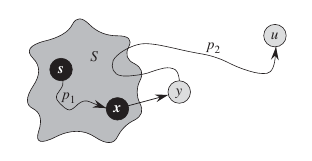
\includegraphics[scale=0.5]{images/sssp_3_1.png}
  \end{figure}
  
  We now claim $y.d = \delta(s,y)$ when $u$ is added to $S$. First, observe that $x \in S$. Then, because we chose $u$ as first vertex for which $u.d \neq \delta(s,u)$ when it is added to $S$, we had $x.d = \delta(s,x)$ when $x$ was added to $S$. Edge $(x,y)$ was relaxed at that time, and the claim follows from the convergence property.

  We can now obtain a contradiction to prove that $u.d = \delta(s,u)$. Because $y$ lies before $u$ on the shortest path from $s$ to $u$ and all edge weights are non-negative (notably those on path $p_2$), we have $\delta(s,y) \leq \delta(s,u)$, and thus

  \bee
  y.d = \delta(s,y) \leq \delta(s,u) \leq u.d
  \eee

  where the last inequality follows from the upper-bound property. But because both vertices $u$ and $y$ were in $V-S$ when $u$ was chosen in line $6$, we have $u.d \leq y.d$. Thus, the two inequalities are in fact equalities, giving $y.d = \delta(s,y) = \delta(s,u) = u.d$. Consequently, $u.d = \delta(s,u)$, which contradicts our choice of $u$. We conclude that $u.d = \delta(s,u)$ when $u$ is added to $S$, and that equality is maintained at all time thereafter.
  
  At \emph{termination}, $Q = \o$ wich implies $S = V$. Thus, $u.d = \delta(s,u)$ for all vertices $u \in V$.
  
\end{proof}

\begin{theorem} If we run Dijkstra's algorithm on a weighted, directed graph $G$ with non-negative weight function $w$ and source $s$, then at termination, the predecessor subgraph $G_\pi$ is a shortest-paths tree rooted at $s$.
\end{theorem}

\begin{proof}
  This follows from the previous theorem and the predecessor-subgraph property.
\end{proof}

%%% Local Variables:
%%% mode: latex
%%% TeX-master: "journal"
%%% End:
